\documentclass[11pt]{article}

% --- Portable, arXiv-friendly preamble (no proprietary fonts, no absolute paths) ---
\usepackage[T1]{fontenc}
\usepackage[utf8]{inputenc}
\usepackage[hmargin=1in,vmargin=1in]{geometry}
\usepackage{amsmath,amssymb}
\usepackage{booktabs}
\usepackage{graphicx}
\graphicspath{{figures/}}
\usepackage{xcolor}
\usepackage{caption}
\usepackage[numbers,sort&compress]{natbib}
\usepackage{hyperref}
\hypersetup{colorlinks=true,linkcolor=blue!50!black,citecolor=blue!50!black,urlcolor=blue!50!black}
\usepackage{url}
\usepackage{microtype}

\newcommand{\reduc}[1]{\ensuremath{#1\%}}

\title{\textbf{Training Corpus Matters: Byte-Level BPE Compression\\ on Cloud and Technical Documentation}\\
\large A controlled, byte-matched case study measuring tokenizer compression, not model quality}

% Author metadata is a PLACEHOLDER pending confirmation
% (see publication/AUTHOR_INPUTS_REQUIRED.md). Do not treat as final.
\author{%
  \texttt{$\langle$AUTHOR NAME$\rangle$}\thanks{Author, affiliation, and any employer
  relationship are placeholders pending confirmation; see the repository's
  \texttt{publication/AUTHOR\_INPUTS\_REQUIRED.md}. This is an independent research
  artifact using only public documentation; it does not represent Microsoft's
  position and implies no endorsement.}\\
  \texttt{$\langle$AFFILIATION$\rangle$}
}
\date{2026}

\begin{document}
\maketitle

\begin{abstract}
General-purpose tokenizers may allocate vocabulary inefficiently for specialized
technical documentation, increasing sequence length. We present a controlled,
CPU-only case study of how training-corpus composition affects byte-level BPE
compression on unseen documentation. We hold the tokenizer algorithm,
pre-tokenizer, decoder, normalization, special tokens, vocabulary size, and
training-data budget fixed. Using byte-matched 32\,MiB corpora, we train
General-English, Azure-documentation, and 50/50 Mixed tokenizers with 8K, 16K,
and 32K vocabularies and evaluate them on nine leakage-controlled held-out
datasets. On an unseen cross-service Azure holdout containing 964 documents from
five wholly held-out services, the 16K Azure tokenizer uses \reduc{36.68} fewer
tokens per 1{,}000 UTF-8 bytes than the matched General tokenizer (95\%
paired-bootstrap CI $[35.77\%, 37.62\%]$; document win rate $1.000$). However, it
uses \reduc{34.75} more tokens on held-out general English. The 50/50 Mixed
tokenizer achieves a \reduc{34.21} reduction on the Azure holdout, retaining
\reduc{93.3} of the Azure-only tokenizer's in-domain gain, while using only
\reduc{4.39} more tokens on general English. The in-domain reduction is stable
across the evaluated vocabulary sizes, persists on prose-dominant content, and
transfers partially to other Microsoft and external Kubernetes documentation. We
evaluate tokenizer compression and CPU tokenization throughput only. We make no
claims about model quality, inference latency, GPU throughput, or realized cost.
We release code, pinned source manifests, per-document measurements, and a
machine-verified claim registry; raw source corpora are not redistributed.
\end{abstract}


\section{Introduction}
\label{sec:intro}

Language models read text as \emph{tokens}, and a tokenizer's vocabulary
determines how many tokens a given string becomes. Because sequence length drives
context consumption and per-token accounting, a tokenizer that fragments a domain's
recurring strings---resource identifiers, command flags, paths, configuration
keys---into many pieces imposes a standing overhead on that domain. Subword
tokenizers such as byte-pair encoding (BPE) \citep{sennrich2016bpe}, WordPiece
\citep{schuster2012wordpiece}, and Unigram/SentencePiece
\citep{kudo2018subword,kudo2018sentencepiece} learn their inventories from a
training corpus, so the corpus composition shapes which strings are cheap.

Technical documentation is a useful domain to study this effect: it mixes natural
language with dense, repetitive technical syntax, and large, permissively licensed
corpora exist. Azure documentation is a useful controlled case---sizable,
public, and internally varied across services---so that we can hold out whole
services for genuinely unseen evaluation. Crucially, in-domain gains must be
reported \emph{with} out-of-domain regressions: a tokenizer specialized to one
domain is expected to compress other text worse, and a practical deployment may
prefer a mixed tokenizer that balances the two.

Existing production tokenizers (e.g., \texttt{tiktoken}
\citep{openai2026tiktoken}) differ from one another in training data, vocabulary
size, normalization, and algorithm simultaneously, so comparing them cannot
isolate the effect of the \emph{training corpus} alone. We therefore run a
controlled experiment: identical byte-level BPE tokenizers that differ only in
their training corpus, trained on byte-matched budgets, with leakage-controlled
held-out evaluation.

This paper measures \emph{tokenization compression only}. It does not train or
evaluate a language model, and makes no claim about model quality, accuracy,
reasoning, inference latency, GPU throughput, or realized cost. Our contributions
are:

\begin{enumerate}
  \item A controlled corpus-composition study with matched byte budgets and fixed
  byte-level BPE configuration (General vs Azure vs Mixed, at 8K/16K/32K).
  \item Cross-service and cross-repository held-out evaluation with explicit
  leakage controls (whole-service holdout, exact and near-duplicate removal,
  cross-corpus near-duplicate filtering).
  \item An analysis of the specialization--generalization tradeoff via a 50/50
  Mixed tokenizer.
  \item Content-type, vocabulary-size, coverage, transfer, and CPU-runtime
  analyses, separating compression from runtime.
  \item A reproducible artifact with source locks, raw per-document results, and a
  machine-verified claim registry in which every reported number is reconciled
  against its source file.
\end{enumerate}

\section{Related work}
\label{sec:related}

We organize related work by methodological relationship to this study rather than
as a list of results.

\paragraph{Subword tokenization foundations.}
BPE for open-vocabulary neural machine translation \citep{sennrich2016bpe},
WordPiece \citep{schuster2012wordpiece}, subword regularization and Unigram
language-model tokenization \citep{kudo2018subword}, and SentencePiece
\citep{kudo2018sentencepiece} define the tokenizer families and the
open-vocabulary motivation; byte-level BPE \citep{radford2019gpt2} and
WordPiece-based encoders \citep{devlin2019bert} are widely deployed. We do not
introduce a new tokenizer algorithm; we vary the training corpus within a fixed
byte-level BPE design.

\paragraph{Byte-level BPE and implementation baselines.}
Byte-level BPE \citep{radford2019gpt2} and its production implementations
\citep{openai2026tiktoken,huggingface2026tokenizers} provide robust,
full-coverage tokenization. We use one such implementation for the controlled
tokenizers and treat production \texttt{tiktoken} encodings as observational
baselines.

\paragraph{Domain-specific tokenizers and vocabularies.}
Prior work builds domain-specific vocabularies or tokenizers for scientific
\citep{beltagy2019scibert}, legal \citep{chalkidis2020legalbert}, legal/financial
\citep{bommarito2025kl3m}, and code \citep{feng2020codebert} corpora, and studies
tokenizer choice for domains \citep{dagan2024tokenizer}. Notably, some
domain-adapted models instead reuse a general-domain tokenizer
\citep{lee2019biobert}, which is precisely the vocabulary-mismatch setting this
line of work motivates. This study targets cloud/technical documentation and
isolates \emph{compression} rather than downstream model quality.

\paragraph{Vocabulary adaptation for existing models.}
A separate line adapts or augments an existing model's tokenizer---adaptive
tokenization \citep{sachidananda2021adaptive}, adaptive BPE and vocabulary
adaptation in fine-tuning \citep{balde2024adaptivebpe,herold2025vocabulary},
general-to-specialized adaptation \citep{liyanage2026adaptbpe}, and
parameter-efficient vocabulary adaptation \citep{balde2026learning}. These methods
modify an existing vocabulary and often evaluate downstream tasks; we instead
train tokenizers from scratch on byte-matched corpora and report intrinsic
compression only, so we make no model-substitution claim.

\paragraph{Pre-tokenization and scaling choices.}
Pre-tokenization \citep{kudo2018sentencepiece,dagan2024tokenizer} and the amount of
tokenizer training data \citep{reddy2025diminishing} both affect the learned
inventory. We fix byte-level BPE design choices and vary corpus composition and
vocabulary size, observing diminishing sensitivity across 8K/16K/32K.

\paragraph{Fertility, compression, and fairness metrics.}
Token counts are corpus- and language-sensitive and can create inequities
\citep{petrov2023unfairness}, motivating metrics beyond raw fertility
\citep{nayeem2025strr} and studies of tokenizer choice
\citep{ali2024tokenizerchoice,rust2021tokenizer}. We adopt tokens per 1{,}000
UTF-8 bytes as the outcome and explicitly avoid downstream quality or fairness
claims.

\paragraph{Leakage and evaluation controls.}
Deduplication improves the integrity of train/eval separation for language
modeling \citep{lee2022dedup}. We apply analogous exact and near-duplicate
controls to tokenizer-compression evaluation.

\medskip
Taken together, prior work establishes that tokenizer inventories are
corpus-sensitive and can affect efficiency and downstream systems. Our
contribution is a controlled, byte-matched, leakage-controlled case study
measuring how that sensitivity manifests as \emph{compression} on technical
documentation, including the tradeoff between full specialization and mixed-domain
training. This work sits primarily in the ``trained from scratch on domain data''
and ``fertility/compression measurement'' categories above.

\section{Research questions and hypotheses}
\label{sec:rq}

We pre-registered the hypotheses before inspecting the full results (repository
file \texttt{research/EXPERIMENT\_SPEC.md}).

\begin{itemize}
  \item \textbf{RQ1.} Under matched conditions, does Azure-domain training reduce
  token count on unseen Azure services relative to general-English training?
  \item \textbf{RQ2.} What general-English regression accompanies full
  specialization?
  \item \textbf{RQ3.} Does a 50/50 Mixed corpus preserve most of the in-domain
  gain while limiting the regression?
  \item \textbf{RQ4.} Does the effect transfer to other technical-documentation
  domains?
  \item \textbf{RQ5.} Is the effect stable across 8K, 16K, and 32K vocabularies?
  \item \textbf{RQ6.} Does the effect persist on prose, rather than being explained
  only by code and markup?
  \item \textbf{RQ7.} How do compression and CPU tokenizer throughput relate?
\end{itemize}

\paragraph{Primary hypothesis.} At a fixed byte-level BPE algorithm, vocabulary
size, training-byte budget, normalization, sampling, and evaluation set, an
Azure-trained tokenizer produces fewer tokens per 1{,}000 UTF-8 bytes on the Azure
cross-service holdout than a byte-matched General tokenizer.

\paragraph{Null hypothesis.} After those controls, the Azure- and General-trained
tokenizers do not differ in token count on the held-out set, i.e.\ the point
estimate of the relative reduction is $\le 0$ or its 95\% paired-bootstrap CI is
compatible with no positive reduction.

\section{Data}
\label{sec:data}

All sources are public and pinned by exact commit or dataset revision (repository
file \texttt{data/manifests/sources.lock.json}); raw source text is not
redistributed. Table~\ref{tab:datasets} summarizes the sources; per-source
licenses, attribution, and acquisition commands are in Appendix~\ref{app:data}.

\begin{table}[t]
\centering
\caption{Public sources, roles, retained Markdown file counts, and licenses.
Sources are pinned by commit; raw text is not redistributed.}
\label{tab:datasets}
\small
\begin{tabular}{llrl}
\toprule
\textbf{Source} & \textbf{Role} & \textbf{Files} & \textbf{License} \\
\midrule
MicrosoftDocs/azure-docs & train (anchor) & 5,340 & CC-BY-4.0 \\
MicrosoftDocs/architecture-center & eval (transfer) & 220 & CC-BY-4.0 \\
MicrosoftDocs/azure-devops-docs & eval (transfer) & 220 & CC-BY-4.0 \\
MicrosoftDocs/sql-docs & eval (transfer) & 220 & CC-BY-4.0 \\
MicrosoftDocs/fabric-docs & eval (transfer) & 150 & CC-BY-4.0 \\
MicrosoftDocs/microsoft-365-docs & eval (transfer) & 200 & CC-BY-4.0 \\
kubernetes/website & eval (external) & 250 & CC-BY-4.0 \\
Salesforce/wikitext & train+eval & 14,900 & CC-BY-SA-3.0 \\
\bottomrule
\end{tabular}

\end{table}

\paragraph{Training corpora.} Three byte-matched corpora of 33{,}554{,}432 UTF-8
bytes each: \emph{General} (Wikipedia-derived English, WikiText-103-raw),
\emph{Azure} (20 service directories of \texttt{MicrosoftDocs/azure-docs},
$3{,}799$ documents after deduplication and holdout), and \emph{Mixed}, a
deterministic document-by-document 50/50 interleave. Corpora are matched on
cleaned bytes, not document count.

\paragraph{Evaluation corpora.} Nine held-out sets: the Azure cross-service
holdout (five whole services never seen in training, the \emph{principal} set,
$964$ documents), an Azure same-service holdout, four Microsoft transfer sets
(architecture, DevOps, data, broad-enterprise), one external technical control
(Kubernetes website documentation), a held-out general-English set, and a
diagnostic synthetic set.

\paragraph{Cleaning, classification, and leakage control.} Documents are decoded
as UTF-8, NFC-normalized (no lowercasing or accent stripping), stripped of front
matter and build directives, segmented, and classified into content types by a
rule-based classifier. Exact duplicates (SHA-256) and MinHash near-duplicates are
removed from Azure before splitting; the General corpus is exact-deduplicated
before the train/eval split ($134$ documents removed); and evaluation items that
are near-duplicates of any training document are removed ($9$ items). Whole Azure
services are held out so the principal evaluation is service-disjoint from
training. We do not reproduce source-document text beyond minimal illustrative
tokens.

\section{Methodology}
\label{sec:method}

\paragraph{Controlled tokenizers (Track A).} We train byte-level BPE tokenizers
\citep{radford2019gpt2} with the Hugging Face \texttt{tokenizers} implementation
\citep{huggingface2026tokenizers}, holding fixed: a byte-level pre-tokenizer and
matching decoder, a full byte-level initial alphabet (so ordinary text never
produces an unknown token), Unicode NFC normalization without lowercasing or
accent stripping, the special-token set, and a minimum merge frequency of two.
The only variable is the training corpus (General, Azure, Mixed). Vocabulary sizes
are $8{,}192$, $16{,}384$, and $32{,}768$ (special tokens count toward the size),
giving nine controlled tokenizers. Sampling, splitting, and the bootstrap are
driven by a single seed ($20{,}260{,}709$). Corpora are sampled deterministically
to exactly $33{,}554{,}432$ bytes each; the Mixed corpus interleaves Azure and
General documents 50/50 by bytes. Table~\ref{tab:matrix} lists the design.

\begin{table}[t]
\centering
\caption{Controlled experimental design. Only the training corpus is manipulated;
all other factors are held fixed within a comparison.}
\label{tab:matrix}
\small

\begin{tabular}{lll}
\toprule
\textbf{Factor} & \textbf{Levels} & \textbf{Held constant} \\
\midrule
Training corpus (manipulated) & General, Azure, Mixed 50/50 & --- \\
Vocabulary size & 8{,}192 / 16{,}384 / 32{,}768 & within a comparison \\
Algorithm & byte-level BPE & implementation, pre-tokenizer, decoder \\
Training budget & 33,554,432 UTF-8 bytes & byte-matched across corpora \\
Normalization & Unicode NFC & no lowercasing, no accent stripping \\
Seed & 20260709& sampling, splitting, bootstrap \\
\bottomrule
\end{tabular}

\end{table}

\paragraph{Observational baselines (Track B).} We also encode the evaluation sets
with production \texttt{tiktoken} encodings (\texttt{r50k\_base},
\texttt{cl100k\_base}, \texttt{o200k\_base}) \citep{openai2026tiktoken}. These
differ from Track A and from one another in training data, vocabulary size,
normalization, and intended model, so they are reported separately and are not a
controlled comparison.

\paragraph{Primary metric.} For a tokenizer $T$ and evaluation corpus $D$,
\begin{equation}
\mathrm{tpk}(T, D) = 1000 \cdot \frac{\mathrm{tokens}(T, D)}{\mathrm{bytes}_{\text{UTF-8}}(D)},
\end{equation}
tokens per $1{,}000$ UTF-8 bytes (lower is more compression), reported both
\emph{micro} (over all bytes) and \emph{macro} (mean of per-document ratios).
The primary effect size is the relative reduction of a specialized tokenizer $A$
versus the matched General tokenizer $G$,
\begin{equation}
\Delta(A \text{ vs } G, D) = 100 \cdot \frac{\mathrm{tpk}(G, D) - \mathrm{tpk}(A, D)}{\mathrm{tpk}(G, D)},
\end{equation}
where \emph{positive} $\Delta$ means the specialized tokenizer uses \emph{fewer}
tokens. Secondary metrics include characters/bytes per token, tokens per
whitespace word, identifier fragmentation, vocabulary utilization, exact
round-trip and unknown-token rates, and CPU throughput.

\paragraph{Statistics.} Token counts are deterministic; uncertainty comes from the
sampled documents. We use a paired bootstrap over documents ($10{,}000$ resamples;
the same documents resampled for both tokenizers), reporting 95\% confidence
intervals for $\Delta$, a document-level win rate, and stratification by
evaluation set, content type, and repository.

\paragraph{Runtime.} CPU tokenizer throughput is measured separately from
compression, with a fixed thread count, warm-up, five measured rounds, randomized
tokenizer order per round, identical documents and batches, and serialized
execution, on an Apple M3 Pro (12 cores, macOS). This is CPU tokenizer throughput,
not model-serving throughput.

\paragraph{Verification.} An automated gate re-checks byte-matching, leakage
controls, exact round-trip and unknown-token counts, totals reconciliation,
provenance completeness, artifact-distribution policy, and source pinning without
retraining. Every number in this paper is additionally reconciled against its
source file by a claim registry (Appendix~\ref{app:verify}).

\section{Results}
\label{sec:results}

We report the 16K slice unless stated. Positive relative reduction means the
specialized tokenizer uses fewer tokens. All values are reconciled against source
files by the claim registry (Appendix~\ref{app:verify}).

\paragraph{Primary result.} On the Azure cross-service holdout (five whole
held-out services, $n=964$ documents), the Azure tokenizer uses $240.18$ tokens
per $1{,}000$ UTF-8 bytes versus $379.30$ for the byte-matched General tokenizer,
a relative reduction of \reduc{36.68} (95\% paired-bootstrap CI
$[35.77\%, 37.62\%]$; document win rate $1.000$). Table~\ref{tab:main} and
Figure~\ref{fig:primary} summarize the result and its stability across
vocabulary sizes.

\begin{table}[t]
\centering
\caption{Main results at 16K: token reduction (\%) relative to the byte-matched
General tokenizer on the Azure cross-service holdout and on held-out general
English. Positive $=$ fewer tokens.}
\label{tab:main}
\small

\begin{tabular}{lrr}
\toprule
\textbf{Tokenizer (16K)} & \textbf{Azure cross-service} & \textbf{General English} \\
 & \textbf{reduction (\%)} & \textbf{reduction (\%)} \\
\midrule
Azure & $+36.68$ & $-34.75$ \\
Mixed (50/50) & $+34.21$ & $-4.39$ \\
General & $0$ (ref.) & $0$ (ref.) \\
\midrule
\multicolumn{3}{l}{\footnotesize Azure primary 95\% CI $[35.77, 37.62]$, win rate 1.0, $n=964$.} \\
\multicolumn{3}{l}{\footnotesize Positive $=$ specialized tokenizer uses fewer tokens per 1{,}000 UTF-8 bytes.} \\
\bottomrule
\end{tabular}

\end{table}

\begin{figure}[t]
\centering
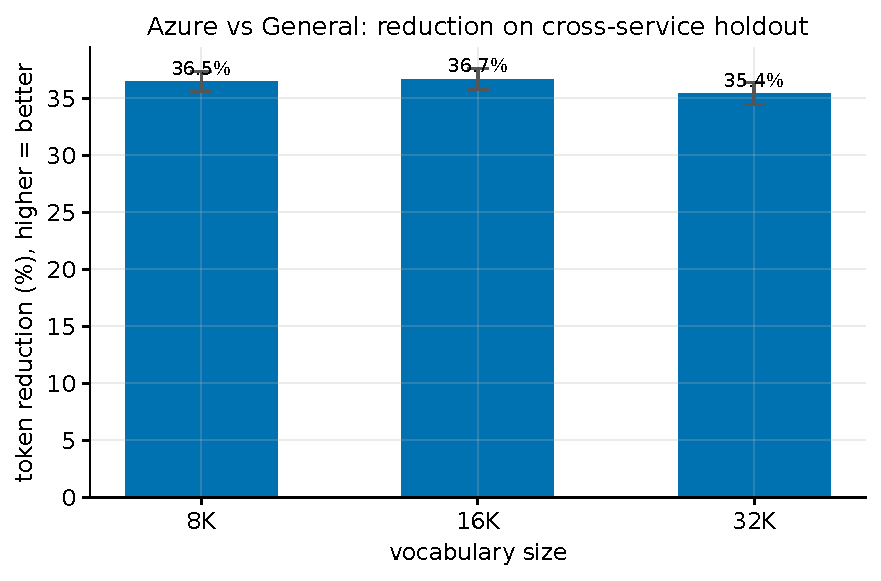
\includegraphics[width=0.62\linewidth]{fig01_primary.pdf}
\caption{Relative token reduction (\%) of the Azure vs byte-matched General
tokenizer on the Azure cross-service holdout, by vocabulary size, with 95\%
paired-bootstrap confidence intervals. Higher is better.}
\label{fig:primary}
\end{figure}

\paragraph{General-English regression (RQ2).} Full specialization has a cost: on
held-out general English the Azure tokenizer uses \reduc{34.75} more tokens than
General (95\% CI $[34.40\%, 35.10\%]$ more)---the direction reverses on
out-of-domain text.

\paragraph{Mixed-tokenizer tradeoff (RQ3).} The 50/50 Mixed tokenizer achieves a
\reduc{34.21} reduction on the Azure holdout---retaining \reduc{93.3} of the
Azure-only tokenizer's in-domain gain---while using only \reduc{4.39} more tokens
on held-out general English (Figure~\ref{fig:tradeoff}).

\begin{figure}[t]
\centering
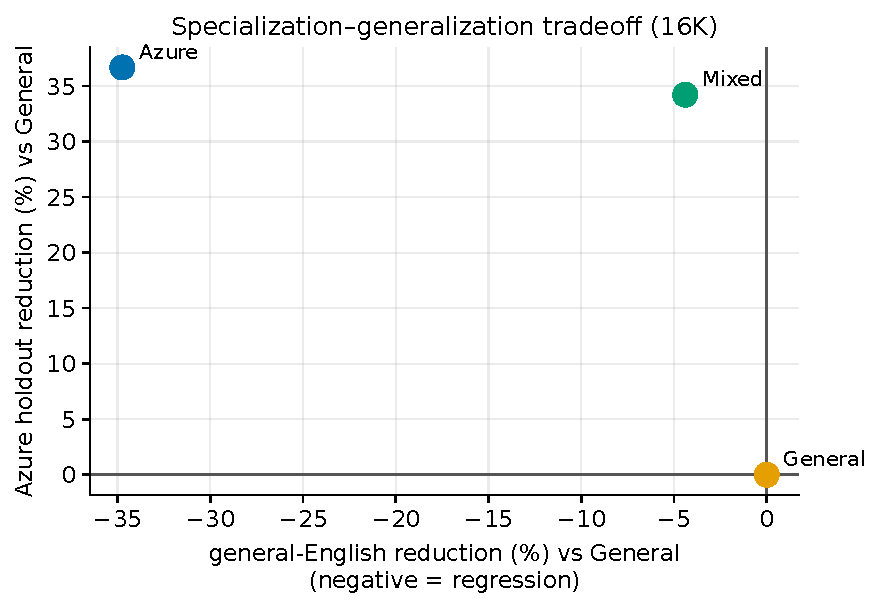
\includegraphics[width=0.6\linewidth]{fig02_tradeoff.pdf}
\caption{Specialization--generalization tradeoff at 16K: token reduction (\%)
relative to General on the Azure holdout (y) versus held-out general English (x).
Up and to the right is better on both axes.}
\label{fig:tradeoff}
\end{figure}

\paragraph{Transfer (RQ4).} The advantage decays with domain distance and persists
on non-Microsoft documentation: $+35.03\%$ (Azure same-service), $+32.94\%$
(Microsoft data), $+31.76\%$ (Microsoft DevOps), $+31.18\%$ (Kubernetes,
external), $+26.03\%$ (Microsoft architecture), and $+25.89\%$ (Microsoft
broad-enterprise); all confidence intervals exclude zero. Table~\ref{tab:transfer}
and Figure~\ref{fig:transfer} report transfer with the general-English regression.

\begin{table}[t]
\centering
\caption{Transfer of the Azure vs General reduction (\%, 16K) across evaluation
sets, plus vocabulary-size sensitivity on the principal holdout. Positive $=$
fewer tokens.}
\label{tab:transfer}
\small
\begin{tabular}{lr}
\toprule
\textbf{Evaluation set} & \textbf{Azure vs General reduction (\%)} \\
\midrule
Azure cross-service holdout (principal) & $+36.68$ \\
Azure same-service holdout & $+35.03$ \\
Microsoft data docs & $+32.94$ \\
Microsoft DevOps docs & $+31.76$ \\
Kubernetes (external technical) & $+31.18$ \\
Microsoft architecture docs & $+26.03$ \\
Microsoft broad-enterprise docs & $+25.89$ \\
General English & $-34.75$ \\
\midrule
\multicolumn{2}{l}{\footnotesize Vocabulary sensitivity (principal): 8K $+36.46$, 16K $+36.68$, 32K $+35.41$.} \\
\bottomrule
\end{tabular}

\end{table}

\begin{figure}[t]
\centering
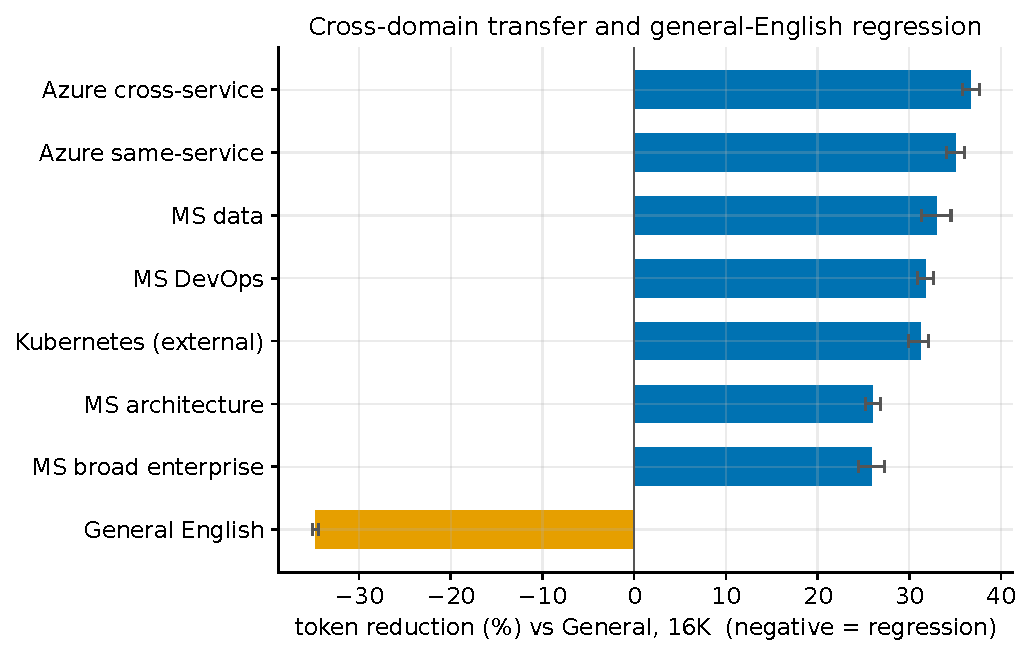
\includegraphics[width=0.72\linewidth]{fig03_transfer.pdf}
\caption{Azure vs General reduction (\%, 16K) across evaluation sets with 95\%
paired-bootstrap CIs. The general-English bar is negative (a regression).}
\label{fig:transfer}
\end{figure}

\paragraph{Vocabulary-size sensitivity (RQ5).} The reduction on the principal
holdout is stable across the tested range: \reduc{+36.46} (8K), \reduc{+36.68}
(16K), \reduc{+35.41} (32K) (Figure~\ref{fig:vocab}), suggesting corpus
composition mattered more than the tested vocabulary range.

\begin{figure}[t]
\centering
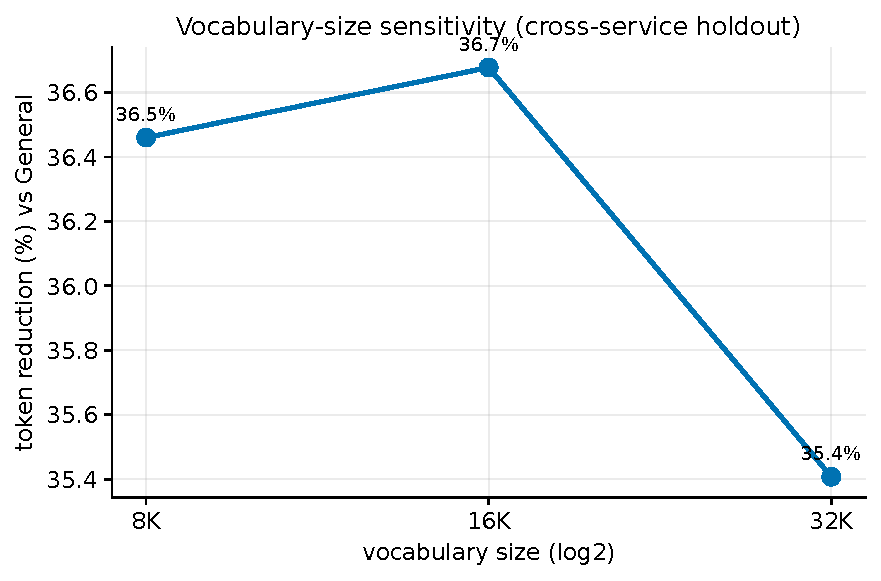
\includegraphics[width=0.58\linewidth]{fig04_vocab.pdf}
\caption{Vocabulary-size sensitivity: Azure vs General reduction (\%) on the
cross-service holdout at 8K/16K/32K.}
\label{fig:vocab}
\end{figure}

\paragraph{Content type (RQ6).} By dominant content type on the principal holdout:
prose-dominant documents ($n=900$) show \reduc{+36.75} (95\% CI
$[35.87\%, 37.63\%]$), headings \reduc{+37.49}, tables \reduc{+44.30}, and inline
code \reduc{+33.28} (Figure~\ref{fig:content}). Because the largest stratum
(prose) still shows a large reduction, the effect is not explained only by code
fences or configuration syntax.

\begin{figure}[t]
\centering
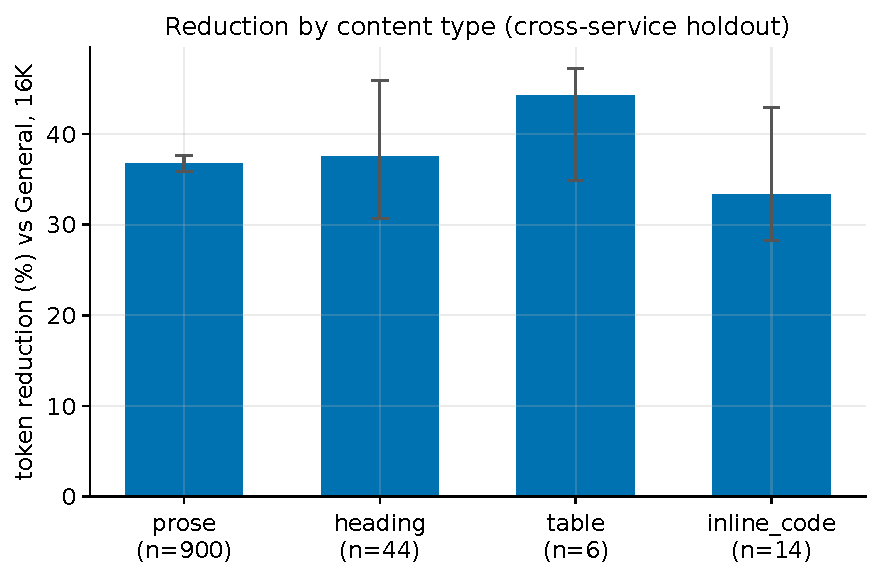
\includegraphics[width=0.58\linewidth]{fig05_content.pdf}
\caption{Reduction by dominant content type on the cross-service holdout (16K),
with 95\% CIs and per-stratum document counts.}
\label{fig:content}
\end{figure}

\paragraph{Coverage and runtime (RQ7).} Across $12$ encoders $\times$ $9$
evaluation sets ($59{,}160$ rows), reconstruction is exact ($100\%$ round-trip)
with zero unknown tokens. Median CPU tokenizer throughput is $5.1$--$5.5$\,MB/s
for the controlled tokenizers and $11.6$--$19.8$\,MB/s for the \texttt{tiktoken}
baselines (Figure~\ref{fig:runtime}); the controlled tokenizers compress more but
run slower on CPU than the production-optimized baselines. Compression and CPU
throughput are distinct dimensions, and CPU throughput is not model-serving
throughput. Table~\ref{tab:runtime} summarizes coverage and runtime.

\begin{table}[t]
\centering
\caption{Coverage and CPU-runtime summary. CPU tokenizer throughput is not
model-serving throughput.}
\label{tab:runtime}
\small

\begin{tabular}{lr}
\toprule
\textbf{Measure} & \textbf{Value} \\
\midrule
Evaluation rows & 59,160 (12 encoders $\times$ 9 sets) \\
Exact round-trip & 100\% \\
Unknown tokens (\texttt{[UNK]}) & 0 \\
CPU throughput, Track A (MB/s) & 5.13--5.47 \\
CPU throughput, Track B \texttt{tiktoken} (MB/s) & 11.61--19.83\\
Automated verification gate & 8/8 \\
\bottomrule
\end{tabular}

\end{table}

\begin{figure}[t]
\centering
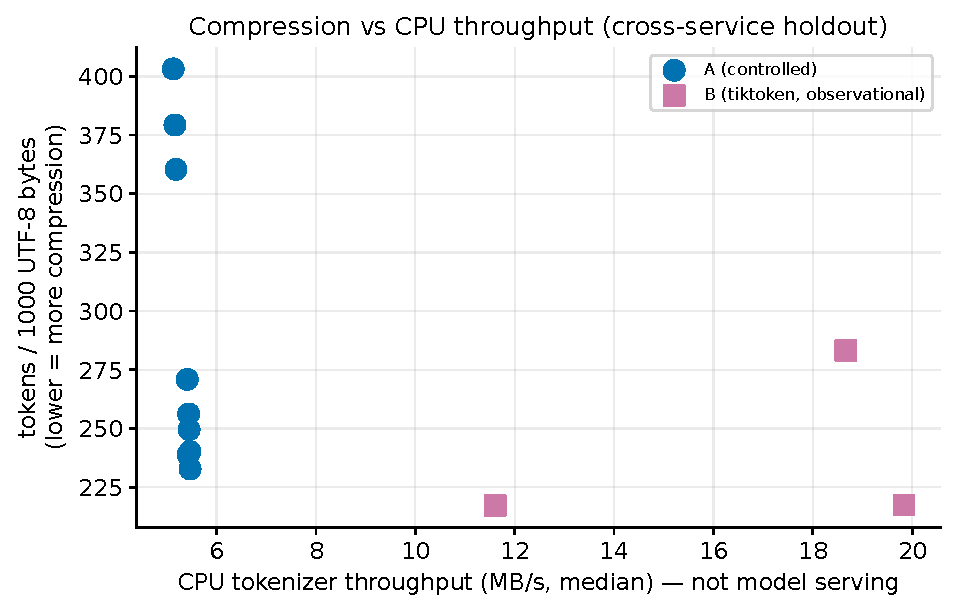
\includegraphics[width=0.62\linewidth]{fig06_runtime.pdf}
\caption{Compression (tokens per $1{,}000$ UTF-8 bytes, lower is better) versus
measured CPU tokenizer throughput on the cross-service holdout. Track A are the
controlled tokenizers; Track B (\texttt{tiktoken}) are observational baselines.}
\label{fig:runtime}
\end{figure}

\section{Analysis and discussion}
\label{sec:analysis}

The results are consistent with the Azure tokenizer allocating vocabulary to
domain-recurring strings and documentation patterns, so that resource-provider
names, command flags, paths, and configuration keys are encoded in fewer pieces.
The mechanism appears in fragmentation and vocabulary-utilization measurements in
the repository: on the principal holdout the Azure tokenizer encodes
resource-provider identifiers, URLs, command flags, and camel/snake identifiers in
fewer tokens than the General tokenizer (for example, roughly half as many tokens
per resource-provider identifier in the repository's fragmentation table), and it
uses a larger fraction of its vocabulary on Azure text.

Several observations bound the interpretation. First, the effect \emph{persists on
prose} (the largest content stratum, $n=900$, still shows \reduc{+36.75}), which
weakens the alternative that gains come only from code fences or configuration
syntax. Second, the advantage \emph{transfers} to non-Microsoft Kubernetes
documentation (\reduc{+31.18}), suggesting overlap in general
technical-documentation style rather than only Azure-specific terminology. Third,
the reduction is \emph{stable across} 8K/16K/32K, suggesting corpus composition
mattered more than the tested vocabulary range. Fourth, the Mixed tokenizer is the
central practical result: it recovers most of the in-domain gain with a small
out-of-domain penalty, which matters when a single tokenizer must serve mixed
traffic.

We are explicit about a design limit: comparing Azure documentation with general
English changes \emph{more than subject domain}. It also changes technical writing
style, markup distribution, identifier density, and document structure. The
transfer and prose-only analyses narrow, but do not fully isolate, Azure-specific
vocabulary from general technical-documentation specialization
(Section~\ref{sec:limits}). Finally, faster compression does not imply faster CPU
tokenization---the controlled tokenizers compress more yet run slower on CPU than
the production baselines---and none of these measurements support any downstream
model claim.

\subsection*{What this study is and is not}

\noindent\fbox{\parbox{0.98\linewidth}{%
\textbf{This study is:} a tokenizer-training and \emph{compression} benchmark; a
controlled comparison of corpus composition; a held-out technical-documentation
evaluation; a study of domain/general tradeoffs; a CPU-only reproducible artifact.

\smallskip
\textbf{This study is not:} an LLM quality evaluation; a model-adaptation method; a
serving or GPU benchmark; a billing study; an endorsement of replacing production
tokenizers; or a claim that fewer tokens always means a better system.%
}}

\section{Limitations}
\label{sec:limits}

We state limitations plainly and do not minimize them.

\paragraph{Training budget and design.} Corpora are byte-matched at a small
$32$\,MiB budget, bounded by the available cleaned Azure training text; absolute
token counts are budget-dependent. The controlled matrix uses a single tokenizer
algorithm (byte-level BPE). Sources are technical documentation, so results may
not extend to chat, source-code repositories, prose, or all enterprise text.

\paragraph{The Azure-versus-general-English confound (most important).} Comparing
Azure documentation with general English changes more than subject domain; it also
changes technical writing style, markup distribution, identifier density, and
document structure. The transfer and prose-only analyses narrow this concern but
do \emph{not} fully isolate Azure-specific vocabulary from general
technical-documentation specialization. A matched general-technical documentation
training control is the priority follow-up (Section~\ref{sec:future}).

\paragraph{Scope of measurement.} We train no language model and evaluate no
downstream task; there is no GPU or serving benchmark. CPU runtime was measured on
a thermally variable laptop, so small runtime differences are not overinterpreted,
and CPU tokenizer throughput is not model-serving throughput.

\paragraph{Data and comparison caveats.} Results are tied to pinned public-source
snapshots that change over time; raw corpora are not redistributed, and
reproduction downloads the pinned sources. Existing production tokenizers (Track
B) are observational, not controlled. Any context-window or token-billing figure
elsewhere is a derived estimate, not a measured GPU or billing outcome. We claim
no universal domain-tokenizer superiority.

\paragraph{Affiliation.} If the author is affiliated with the vendor of the studied
documentation, that relationship is disclosed where applicable; this study uses
only public documentation, is not an official result of that vendor, and implies
no endorsement.

\section{Ethics, licensing, and broader impact}
\label{sec:ethics}

\paragraph{Sources and licensing.} All data are public documentation. Microsoft
documentation sources are used under CC-BY-4.0 (documentation) with MIT code
samples; the Kubernetes website content is CC-BY-4.0; the general-English corpus
(WikiText-103) is Wikipedia-derived under CC-BY-SA. Sources are pinned by commit
and attributed in the repository (\texttt{licenses/}). No user data and no private
content are used.

\paragraph{Redistribution boundaries.} We do not republish raw source corpora;
reproduction downloads the pinned public sources. We release scripts, source
manifests, content hashes, per-document result rows, processed tables, and
figures. The Azure-only tokenizer artifact is redistributable with attribution;
the General and Mixed tokenizers are derived in part from WikiText and are kept
local-use-only pending clarification of the applicable share-alike terms.

\paragraph{Broader impact.} Token-count differences across domains can translate
into uneven context capacity and per-token accounting across users and domains;
studying compression makes such disparities measurable. We caution against
over-reading compression as model quality: fewer tokens is an efficiency property,
not evidence of better understanding, accuracy, or safety.

\paragraph{Environmental scope.} The experiment is CPU-only and trains no language
model; its compute footprint is small (tokenizer training and evaluation complete
in minutes on a laptop).

\paragraph{Code and data availability.} Code, source manifests with pinned
commits, content hashes, per-document result rows, processed tables, figures, and
a machine-verified claim registry are available at
\url{https://github.com/johnsonshi/azure-domain-tokenization}. Raw source corpora
are not redistributed; reproduction downloads the pinned public sources.

\paragraph{Non-endorsement and review.} This is independent research using only
public documentation. The author is affiliated with Microsoft; this work does not
represent the position of Microsoft or any other vendor, is not an official
Microsoft product or result, and implies no endorsement. We make no IRB claim (no
human-subjects data).

\section{Future work}
\label{sec:future}

The priority follow-up is a \emph{matched general-technical documentation} training
control that shares technical style, markup, and identifier density with the Azure
corpus but not its Azure-specific vocabulary, to separate general
technical-documentation specialization from Azure specialization. Beyond that:
(i)~more corpus mixture ratios between the General and Azure extremes;
(ii)~larger training-data budgets to test whether the reduction changes with
scale; (iii)~other tokenizer algorithms (e.g., Unigram, WordPiece) under matched
controls; (iv)~deeper vocabulary-utilization and token-category allocation
analysis; and (v)~temporal holdouts across documentation snapshots.

Separately, and clearly labeled as future GPU/model work not attempted here, one
could integrate an adapted tokenizer into a small model trained from scratch to
measure any downstream effect, and measure real prefill, KV-cache, latency, and
throughput with a compatible model. Evaluating code-heavy and multilingual
technical documentation, and vocabulary-replacement or adaptation methods rather
than full retraining, are additional directions. None of these downstream or
serving results are claimed by the present study.

\section{Conclusion}
\label{sec:conclusion}

Under a controlled, byte-matched comparison at a matched 16K vocabulary, training a
byte-level BPE tokenizer on Azure documentation reduced token count on an unseen
cross-service Azure holdout by \reduc{36.68} relative to a general-English
tokenizer (95\% CI $[35.77\%, 37.62\%]$), with a general-English regression of
\reduc{-34.75}. A 50/50 Mixed tokenizer retained most of the in-domain gain
(\reduc{+34.21}) with a much smaller general-English penalty (\reduc{-4.39}), and
the advantage transferred partially to other Microsoft and external
technical-documentation corpora. These findings concern \emph{tokenization
compression only}, on the evaluated corpora and under the stated controls; they
imply nothing about model output quality, inference latency, GPU throughput, or
cost. The controlled comparison isolates the training corpus, whereas existing
production tokenizers differ along multiple axes and serve only as observational
context. All numbers are reproducible from a released, machine-verified artifact.


\section*{Reproducibility statement}
All results regenerate from a public, version-controlled repository. Every
empirical result value reported in this paper (effect sizes, confidence intervals,
coverage counts, and runtime summaries) is registered in a machine-readable claim
registry (\texttt{publication/claims.yaml}) and re-checked against its
authoritative source file by \texttt{make verify-claims}; experimental constants
(seed, budgets, batch sizes, vocabulary sizes) are recorded in the repository
configs. The analysis-only path (\texttt{make verify},
\texttt{make verify-claims}, \texttt{make figures}, \texttt{make report}) runs from
committed result files without downloading any corpus; full reproduction downloads
the pinned public sources. See Appendix~\ref{app:repro}.

\section*{Data and code availability}
Code, source manifests with pinned commits, content hashes, per-document result
rows, processed tables, and figures are released under the repository's terms.
Raw source corpora are not redistributed; reproduction downloads the pinned public
sources. The Azure-only tokenizer artifact is distributable with attribution; the
General and Mixed (WikiText-derived) tokenizers are local-use-only pending license
review.

\bibliographystyle{plainnat}
\bibliography{references}

\appendix
\section{Experimental matrix}
\label{app:matrix}
The controlled matrix comprises nine tokenizers: General, Azure, and Mixed (50/50)
training corpora crossed with vocabulary sizes $8{,}192$, $16{,}384$, and
$32{,}768$. Within each vocabulary size, the three tokenizers are identical except
for the training corpus; each is trained on exactly $33{,}554{,}432$ UTF-8 bytes.
Track~B adds three observational \texttt{tiktoken} encodings, giving $12$ encoders
evaluated on $9$ held-out sets. Per-tokenizer provenance (configuration hash,
artifact hash, byte counts, merge count, package versions, machine metadata, and
redistribution flag) is recorded in \texttt{artifacts/tokenizers/*.json}.

\section{Dataset details}
\label{app:data}
Table~\ref{tab:datasets} lists sources, roles, retained Markdown file counts, and
licenses. Each source is pinned by exact commit or dataset revision in
\texttt{data/manifests/sources.lock.json}; per-source acquisition commands,
selection method (git sparse checkout, GitHub API blob download, or Hugging Face
parquet), attribution, and redistribution status are in
\texttt{docs/datasets-and-licenses.md} and \texttt{licenses/}. Raw source text is
not redistributed. Microsoft documentation sources are CC-BY-4.0; the Kubernetes
website is CC-BY-4.0; WikiText-103 is Wikipedia-derived under CC-BY-SA and is used
local-use-only.

\section{Additional results}
\label{app:additional}
The repository reports secondary analyses that support the main text:
identifier-fragmentation distributions (mean tokens per resource-provider
identifier, URL/path, command flag, and camel/snake identifier), vocabulary
utilization (fraction of vocabulary used on the principal holdout and occurrence
concentration), and both micro and macro aggregations of the primary metric. These
tables are generated from the committed per-document rows
(\texttt{results/raw/eval\_rows.parquet}) and are listed in
\texttt{results/DATA\_DICTIONARY.md}. All confidence intervals are 95\%
paired-bootstrap intervals over documents ($10{,}000$ resamples), paired at the
document level and stratified by evaluation set, content type, and repository.

\section{Runtime details}
\label{app:runtime}
CPU tokenizer throughput was measured with a fixed thread count, one warm-up round,
five measured rounds, tokenizer order randomized per round, identical documents and
batches (batch sizes $\{1,8,32,128\}$; short/medium/long buckets), and serialized
execution on an Apple M3 Pro (12 cores, macOS). Median throughput was
$5.1$--$5.5$\,MB/s for the controlled tokenizers and $11.6$--$19.8$\,MB/s for the
\texttt{tiktoken} baselines. Runtime was measured on a thermally variable laptop;
small differences are not overinterpreted. This is CPU tokenizer throughput, not
model-serving throughput, and it is reported separately from compression.

\section{Verification and claim registry}
\label{app:verify}
Every numeric statement in this paper is registered in a machine-readable claim
registry (\texttt{publication/claims.yaml}). For each claim the registry records an
extraction specification (source file and column/key), a frozen display value, and
a tolerance; \texttt{make verify-claims} re-extracts each value from its
authoritative result file and fails on any mismatch. An automated experiment gate
(\texttt{make verify}) independently re-checks byte-matching of corpora, leakage
controls, exact round-trip and unknown-token counts ($100\%$ round-trip, zero
unknown tokens across $59{,}160$ rows), totals reconciliation, provenance
completeness, artifact-distribution policy, and source pinning, without retraining.
The independently recomputed primary micro reduction from the per-document rows is
$36.677\%$, matching the reported \reduc{36.68}.

\section{Reproducibility}
\label{app:repro}
The environment is pinned with \texttt{uv} (Python 3.12; \texttt{uv.lock}). Two
paths are supported. \emph{Analysis-only} reproduction runs from committed result
files without downloading any corpus:
\begin{quote}\ttfamily
uv sync; make verify; make verify-claims; make figures; make report
\end{quote}
\emph{Full} reproduction downloads the pinned public sources and recomputes:
\begin{quote}\ttfamily
make acquire-full audit-full train-all evaluate-all; \\
PROFILE=full make analyze report figures verify
\end{quote}
Full reproduction takes roughly $20$--$25$ minutes on an Apple M3 Pro and a
transient ${\sim}2.7$\,GB of disk (a git-ignored source clone plus working data);
the analysis-only path runs in minutes with no downloads. All stochastic steps are
driven by a single seed ($20{,}260{,}709$); the main known nondeterminism is CPU
runtime timing on a thermally variable laptop.


\end{document}
